\documentclass[11pt,a4paper]{article}
\usepackage{aaai}
\usepackage{times}
\usepackage{url}
\usepackage{amsmath,amsfonts,amssymb}
\usepackage{paralist}
\usepackage{color,xcolor}
\usepackage{bm}
\usepackage{multirow}
\usepackage{makecell}
\usepackage{caption}
\usepackage[linesnumbered,lined]{algorithm2e}
\usepackage{todonotes}

% bold x for equations
\newcommand{\rmx}{\mathrm x} 
% used for table headers
\newcommand{\tabh}[1]{\multicolumn{1}{c|}{\textbf{#1}}}  
% used for the top left cell in a table
\newcommand{\tabc}[2]{\multicolumn{1}{|c||}{\multirow{#1}{*}{\textbf{#2}}}} 
% used for denoting the loss symbol with a subscript
\newcommand{\loss}[1]{J_\text{#1}}
% custom author-year citation
\newcommand{\citeay}[1]{\citeauthor{#1} \shortcite{#1}}

% \aclfinalcopy % Un-comment this line for the final submission
%\def\aclpaperid{***} %  Enter the acl Paper ID here

%\setlength\titlebox{5cm}
% You can expand the titlebox if you need extra space
% to show all the authors. Please do not make the titlebox
% smaller than 5cm (the original size); we will check this
% in the camera-ready version and ask you to change it back.
\title{Disentangled Representation Learning for Text Style Transfer}

\author{
	Vineet John \\
	University of Waterloo \\
	{\tt vineet.john@uwaterloo.ca} \\
	\And
	Lili Mou \\
	AdeptMind Research \\
	{\tt doublepower.mou@gmail.com}\\{\tt lili@adeptmind.ai} \\
	\AND
	Hareesh Bahuleyan \\
	University of Waterloo \\
	{\tt hpallika@uwaterloo.ca} \\
	\And
	Olga Vechtomova \\
	University of Waterloo \\
	{\tt ovechtom@uwaterloo.ca} \\
}

\date{}
\begin{document}
\maketitle
\graphicspath{{images/}}
\setcounter{secnumdepth}{2}

\begin{abstract}
	This paper tackles the problem of disentangling the latent variables of style and content in language models.
	We propose a simple, yet effective approach, which incorporates auxiliary objectives: a multi-task classification objective, and dual adversarial objectives for label prediction and bag-of-words prediction, respectively.
	We show, both qualitatively and quantitatively, that the style and content are indeed disentangled in the latent space, using this approach.
	This disentangled latent representation learning method is applied to attribute (e.g. style) transfer on non-parallel corpora.
	We achieve similar content preservation scores compared to previous state-of-the-art approaches, and significantly better style-transfer strength scores.
	Our code is made publicly available for replicability and extension purposes~\footnote{\url{https://github.com/vineetjohn/linguistic-style-transfer}}.
\end{abstract}

% 


\section{Introduction}

The neural network has been a successful learning machine during the past decade due to its highly expressive modeling capability, which is a consequence of multiple layers of non-linear transformations of input features. Such transformations, however, make intermediate features `latent', in that they do not have explicit meaning and are not explainable. Therefore, neural networks are usually treated as black-box machinery.

Disentangling the latent space of neural networks has become an increasingly important research topic. In the image domain, for example, \citeay{chen2016infogan} use adversarial and information maximization objectives to produce interpretable latent representations that can be tweaked to adjust writing style for handwritten digits, as well as lighting and orientation for face models. \citeay{mathieu2016disentangling} utilize a convolutional autoencoder to achieve the same objective. However, this problem is not well explored in natural language processing.

In this paper, we address the problem of disentangling the latent space of neural networks for text generation. Our model is built on an autoencoder that encodes the latent space (vector representation) of a sentence by learning to reconstruct the sentence itself. We would like the latent space to be disentangled with respect to different features, namely, \textit{style} and \textit{content}.

To accomplish this, we propose a simple approach that combines multi-task and adversarial objectives. We artificially divide the latent representation into two parts: style space and content space. We learn model parameters that produce separate style and content latent spaces from the encoded sentence representation. The multi-task objective operates on the style space to ensure it encodes style information. The adversarial style objective, on the contrary, operates on the content space to minimize the predictability of style. In addition, the bag-of-words adversary minimizes the predictability of original words of the sentence in the style space. In this way, the style and content variables can be disentangled from each other.

These representation learning objectives can be directly used for style-transfer in sentence generation~\cite{hu2017toward,shen2017style,fu2017style}, in which a model can generate a sentence with the same content, but a different style. We simply use an autoencoder to encode the content vector of a sentence, but ignore its encoded style vector. Then we infer from the training data, an empirical embedding of the style that we want to transfer. The encoded content vector and the inferred style vector are concatenated and fed to the decoder. Using this grafting technique, we generate a new sentence similar in content but different in style.

We conducted experiments on two customer review benchmark datasets. Both qualitative and quantitative results show that the style vector does contain most style information, whereas the content vector contains little (if any). In the empirical style-transfer evaluations, we achieve significantly better style-transfer strength scores than previous results, while obtaining better or comparable content preservation scores. We also show, using ablation tests, that the auxiliary losses can be combined well, each playing its own role in disentangling the latent space.


\begin{figure}[ht]
	\centering
	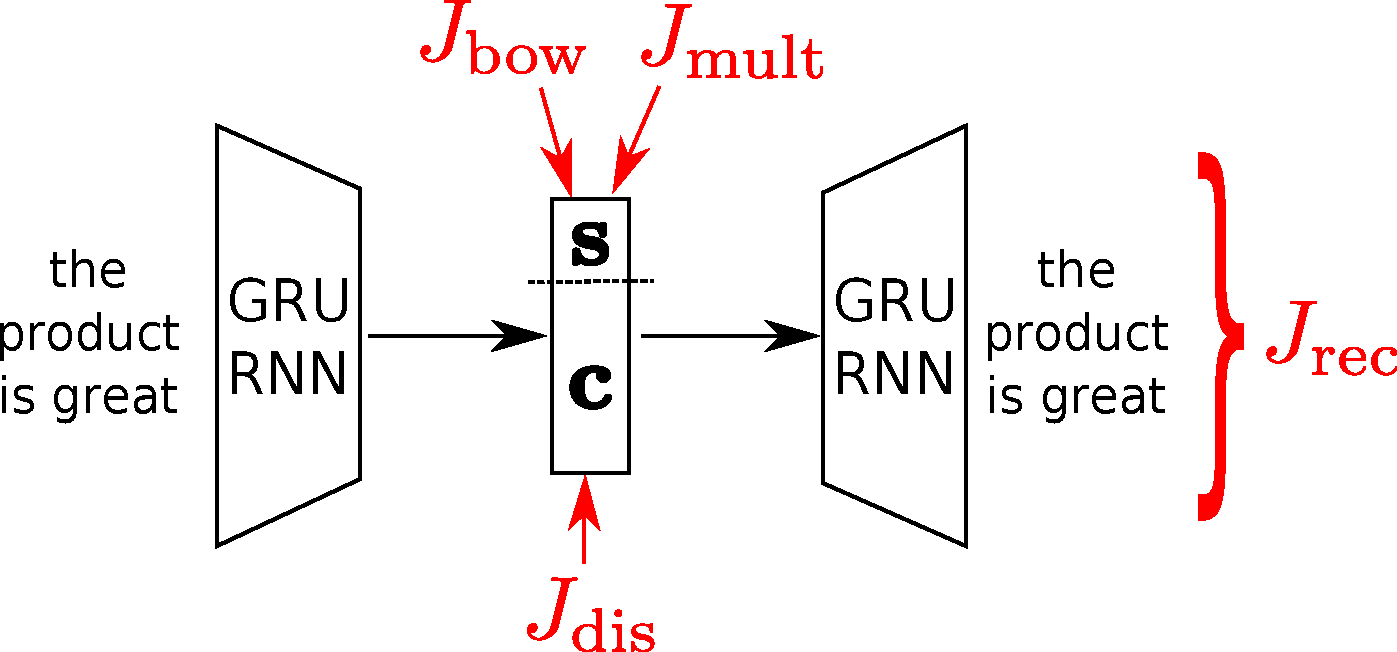
\includegraphics[width=0.8\linewidth]{model-overview-training}
	\caption{Model Training Overview}
	\label{fig:model-training-overview}
\end{figure}
\begin{figure}[ht]
	\centering
	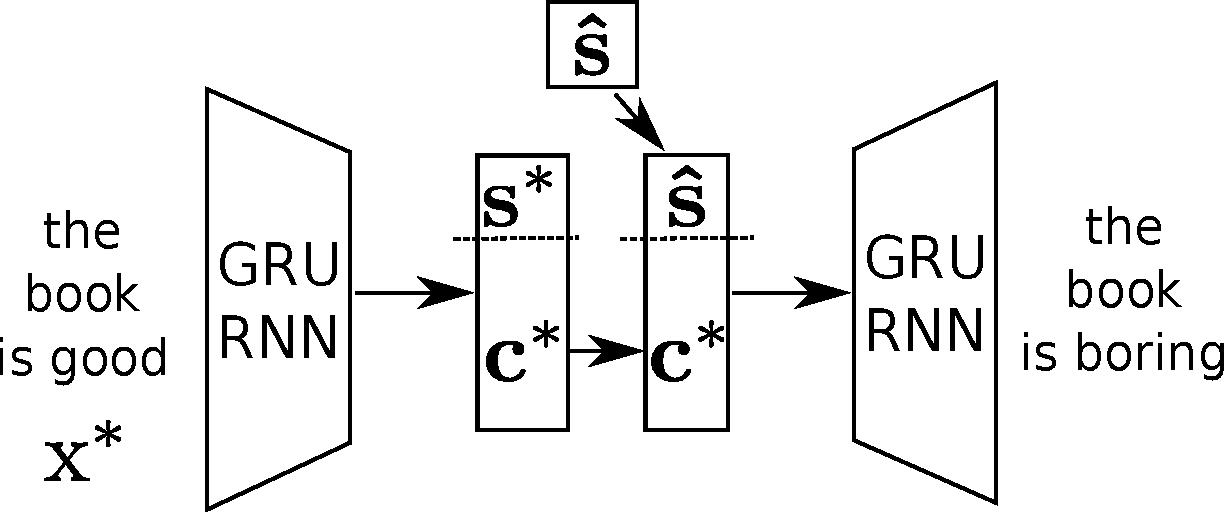
\includegraphics[width=0.8\linewidth]{model-overview-inference}
	\caption{Model Generation Overview}
	\label{fig:model-inference-overview}
\end{figure}


\section{Related Work}

Disentanglement of latent spaces has been explored in the image processing domain in the recent years, and researchers have successfully disentangled rotation features, color features, etc.~\cite{chen2016infogan,luan2017deep}. Some image characteristics (e.g. artistic style) can be captured well by certain statistics, like minimizing the L2 loss between a noise image and a pair of style and content images~\cite{gatys2016image}. In other works, researchers adopt data augmentation techniques to learn a disentangled latent space~\cite{kulkarni2015deep,champandard2016semantic}.

In natural language processing, the definition of `style' itself is vague, and as a convenient starting point, NLP researchers typically treat sentiment as a salient style of text. \citeay{hu2017toward} manage to control the sentiment by using discriminators to reconstruct sentiment and content from generated sentences. However, there is no evidence that the latent space would be disentangled by this reconstruction. \citeay{shen2017style} use a pair of adversarial discriminators to align the recurrent hidden decoder states of (a) original sentences with a given style and (b) sentences transferred to the given style, thereby performing style-transfer. \citeay{fu2017style} propose two approaches, (a) using a style embedding matrix, and (b) using style-specific decoders for style-transfer. They apply an adversarial loss on the encoded space to discourage encoding style in the latent space of an autoencoding model.

Our paper differs from the previous work in that both our style space and content space are encoded from the input. We apply three auxiliary losses to ensure that each space encodes its own information, including a novel bag-of-words adversary that helps disentangle the style space from sentence content. Our disentangled representation learning function can then be directly applied to text style-transfer tasks, as in the aforementioned studies.


\section{Approach}

In this section, we describe our approach in detail. Our model is built upon an autoencoder with a sequence-to-sequence (Seq2Seq) neural network~\cite{sutskever2014sequence}, as described in Subsection \ref{ssec:seq2seq-autoencoder}. Then, we introduce three auxiliary losses: a multi-task classification loss, a style adversarial loss, and a content adversarial loss in Subsections~\ref{ssec:multitask-classification-objective}, \ref{ssec:adversarial-style-objective} and \ref{ssec:adversarial-bow-objective}, respectively. Subsection~\ref{ssec:sentence-generation} presents the approach to transfer style in the context of natural language generation. Figure~\ref{fig:model-training-overview} and Figure~\ref{fig:model-inference-overview} depict the training and style-transferred sentence generation processes of our approach, respectively.

\subsection{Autoencoder} \label{ssec:seq2seq-autoencoder}

An autoencoder encodes an input to a latent vector space, which is usually of a much lower dimensionality than the input data. From this latent space, it decodes the input itself. By doing so, the autoencoder learns salient and compact representations of data. This serves as our primary learning objective. Besides, we also use the autoencoder for text generation in the style-transfer application.

Let $\rmx=(x_1, x_2, \cdots x_n)$ be an input sequence with $n$ tokens. The encoder recurrent neural network (RNN) with gated recurrent units (GRU) \cite{cho2014learning} encodes $\rm x$ and obtains a hidden state $\bm h$. Then a decoder RNN generates a sentence, which ideally should be $\rmx$ itself. Suppose at a time step $t$, the decoder RNN predicts the word $x_t$ with probability $p(x_t|\bm h, x_1\cdots x_{t-1})$, then the deterministic autoencoder (DAE) is trained using a sequence-aggregated cross-entropy loss, given by
\begin{equation}
	\loss{rec}(\bm\theta_E,\bm\theta_D)= -\sum_{t=1}^n \log p(x_t|\bm h, x_1\cdots x_{t-1})
\end{equation}
where $\bm\theta_E$ and $\bm\theta_D$ are the parameters of the encoder and decoder, respectively.

\subsubsection{Variational Autoencoder}

In addition to the deterministic auto-encoding objective presented above, we also implement a variational autoencoder (VAE) \cite{kingma2013auto}. The variational sampling and Kullback-Leibler (KL) divergence \cite{kullback1951information} losses are applicable to both the style space $\bm s$ and the content space $\bm c$, separately. The weights applied to each KL divergence loss are tuned independently as model hyperparameters.

Equation \ref{eqn:vae-rec} shows the reconstruction objective that is minimized in the VAE variant of our model.

\begin{align} \label{eqn:vae-rec}
	\loss{rec}(\bm\theta_E, \bm\theta_D) = \nonumber
	 & - \mathbb{E}_{q_{E}(\bm s|\rmx) q_{E}(\bm c|\rmx)} [\log p(\rmx|\bm s, \bm c)] \nonumber \\
	 & + \lambda_{\text{skl}} KL(q_{E}(\bm s|\rmx)||p(z)) \nonumber                             \\
	 & + \lambda_{\text{ckl}} KL(q_{E}(\bm c|\rmx)||p(z))
\end{align}
where $\lambda_{\text{skl}}$ and $\lambda_{\text{ckl}}$ are the weights for each of the KL divergence terms, and $p(z)$ is the standard normal distribution $\mathcal{N}(0,I)$ that both the encoded style and content distributions are aligned to.

The motivation for using a variational autoencoder variant to compare the base deterministic autoencoder model to, is the property of VAEs that enable them to learn smooth and continuous latent spaces, without many dead zones in the latent space that cannot be decoded from. \citeay{bowman2016generating} show this empirically by using the latent space of a text variational autoencoder to interpolate and generate novel sentences from the latent spaces between two valid sentences from a corpus.

\begin{figure}[t]
	\captionsetup{justification=centering}
	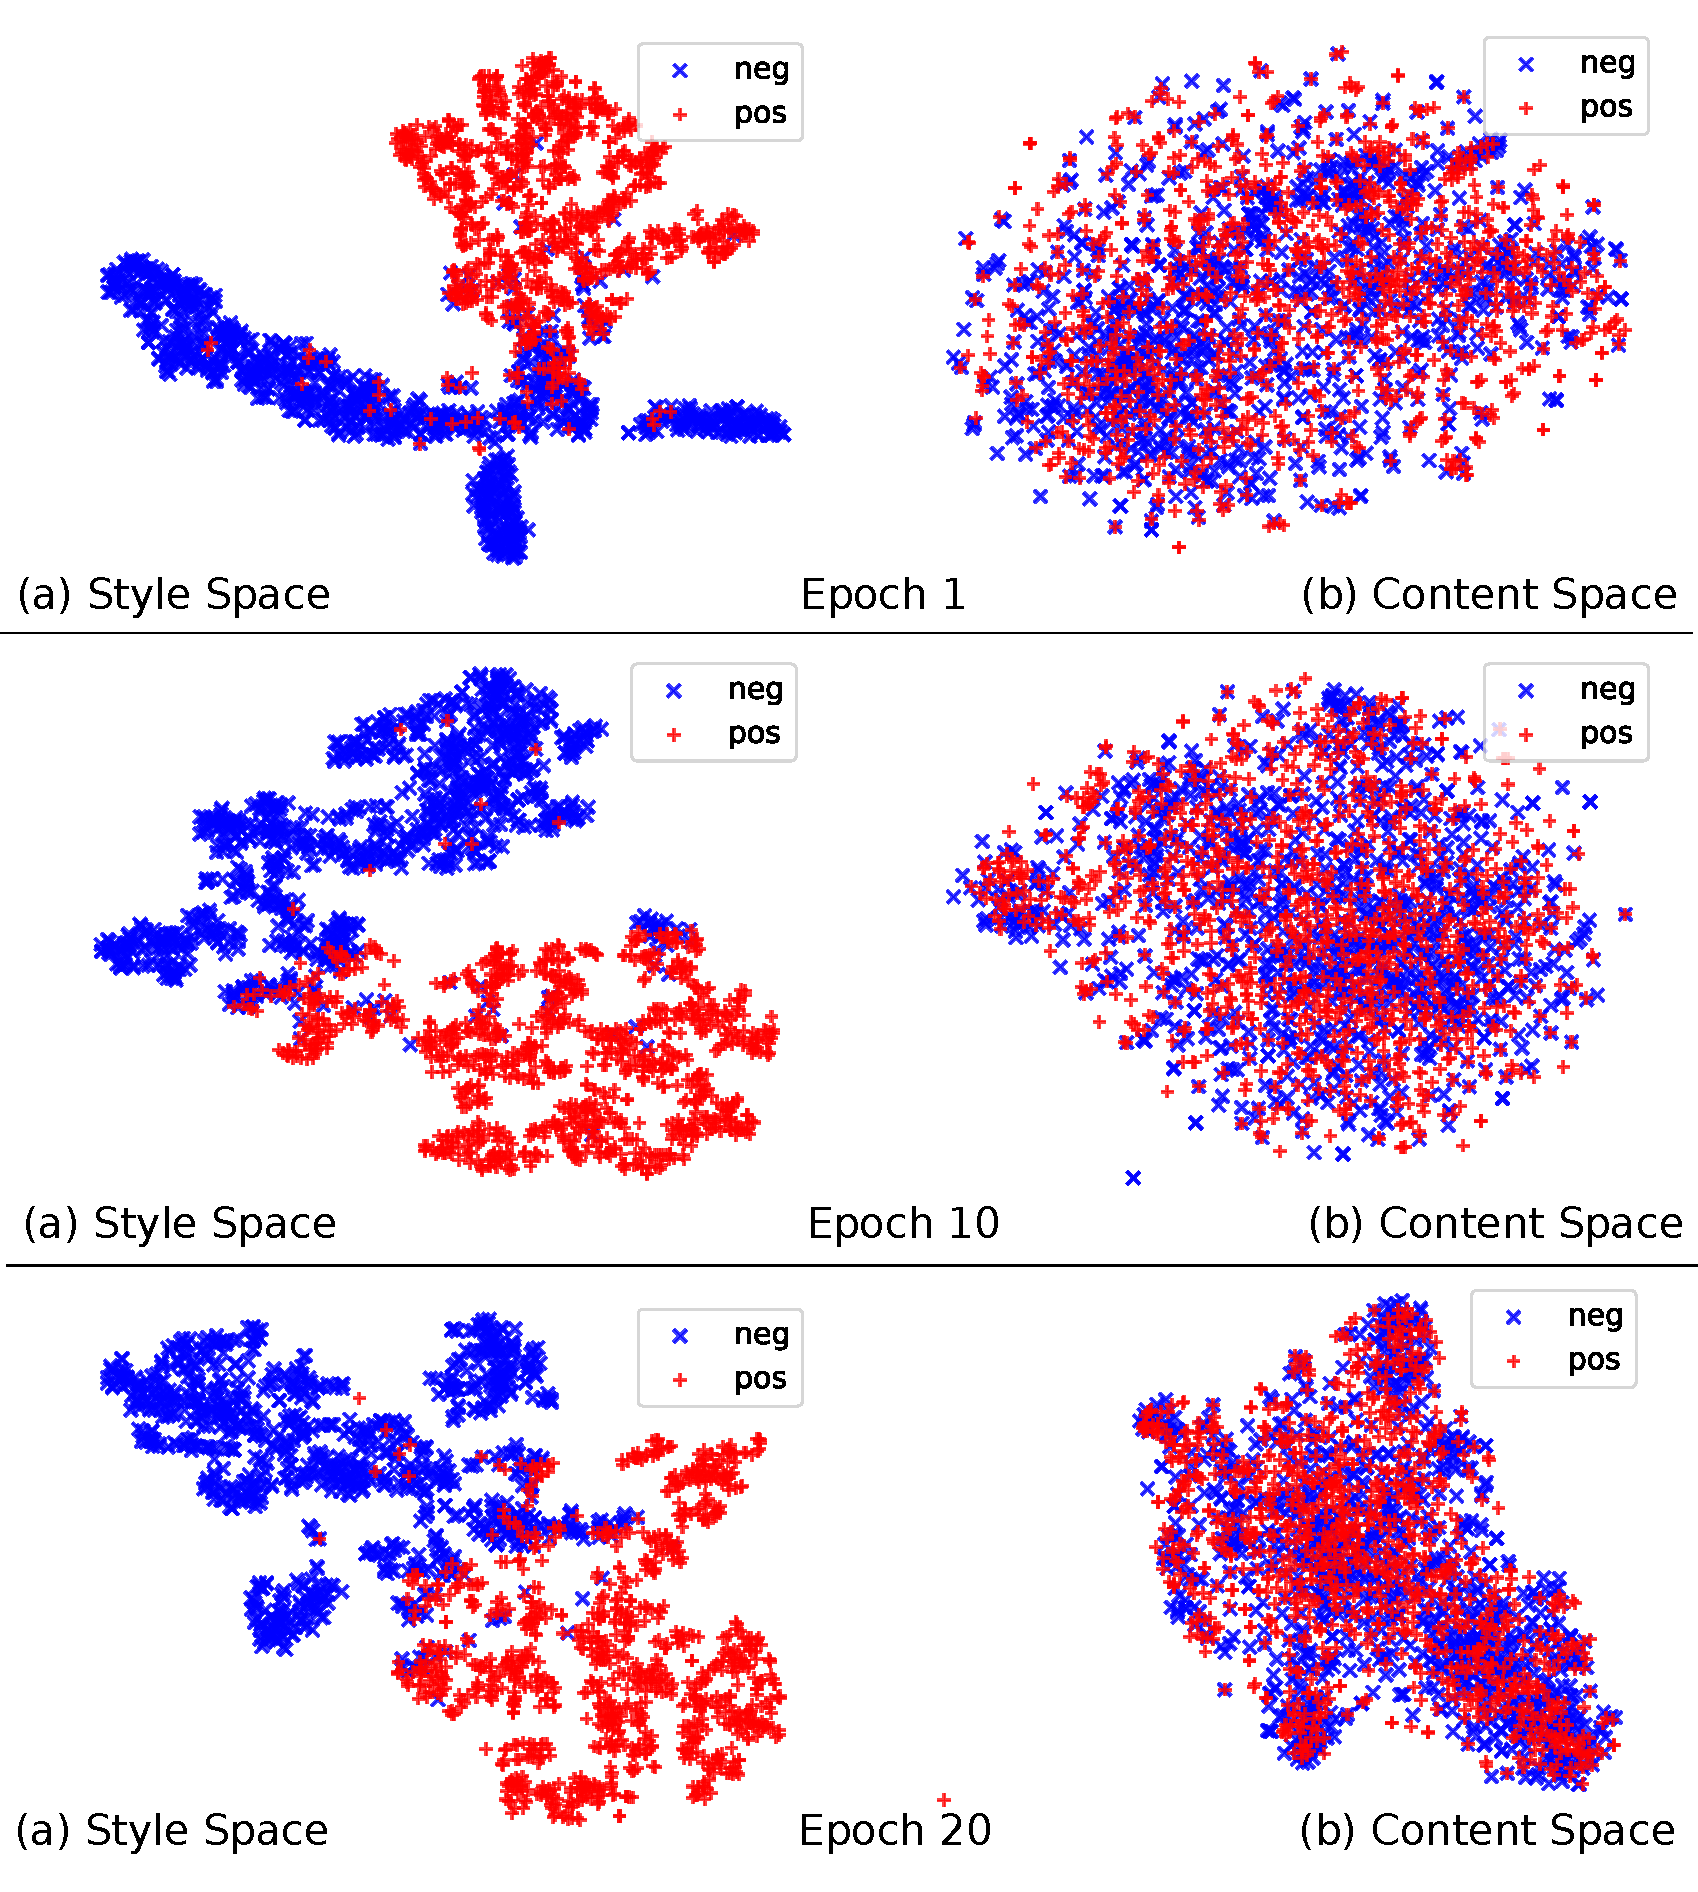
\includegraphics[width=\linewidth]{latent-spaces-dae}
	\caption{t-SNE Plots: Deterministic Autoencoder}
	\label{fig:dae-tsne}
\end{figure}

Since this objective is used to train the model to reconstruct $\rmx$, it is also called the \textit{reconstruction loss}. Besides the above reconstruction loss, we design three auxiliary losses to disentangle the latent space $\bm h$. In particular, we hope that $\bm h$ can be separated into two spaces $\bm s$ and $\bm c$, representing style and content respectively, i.e., $\bm h = [\bm s ; \bm c]$, where $[\cdot;\cdot]$ denotes concatenation. This is accomplished by the auxiliary losses described in the subsequent sections.


\begin{figure}[t]
	\captionsetup{justification=centering}
	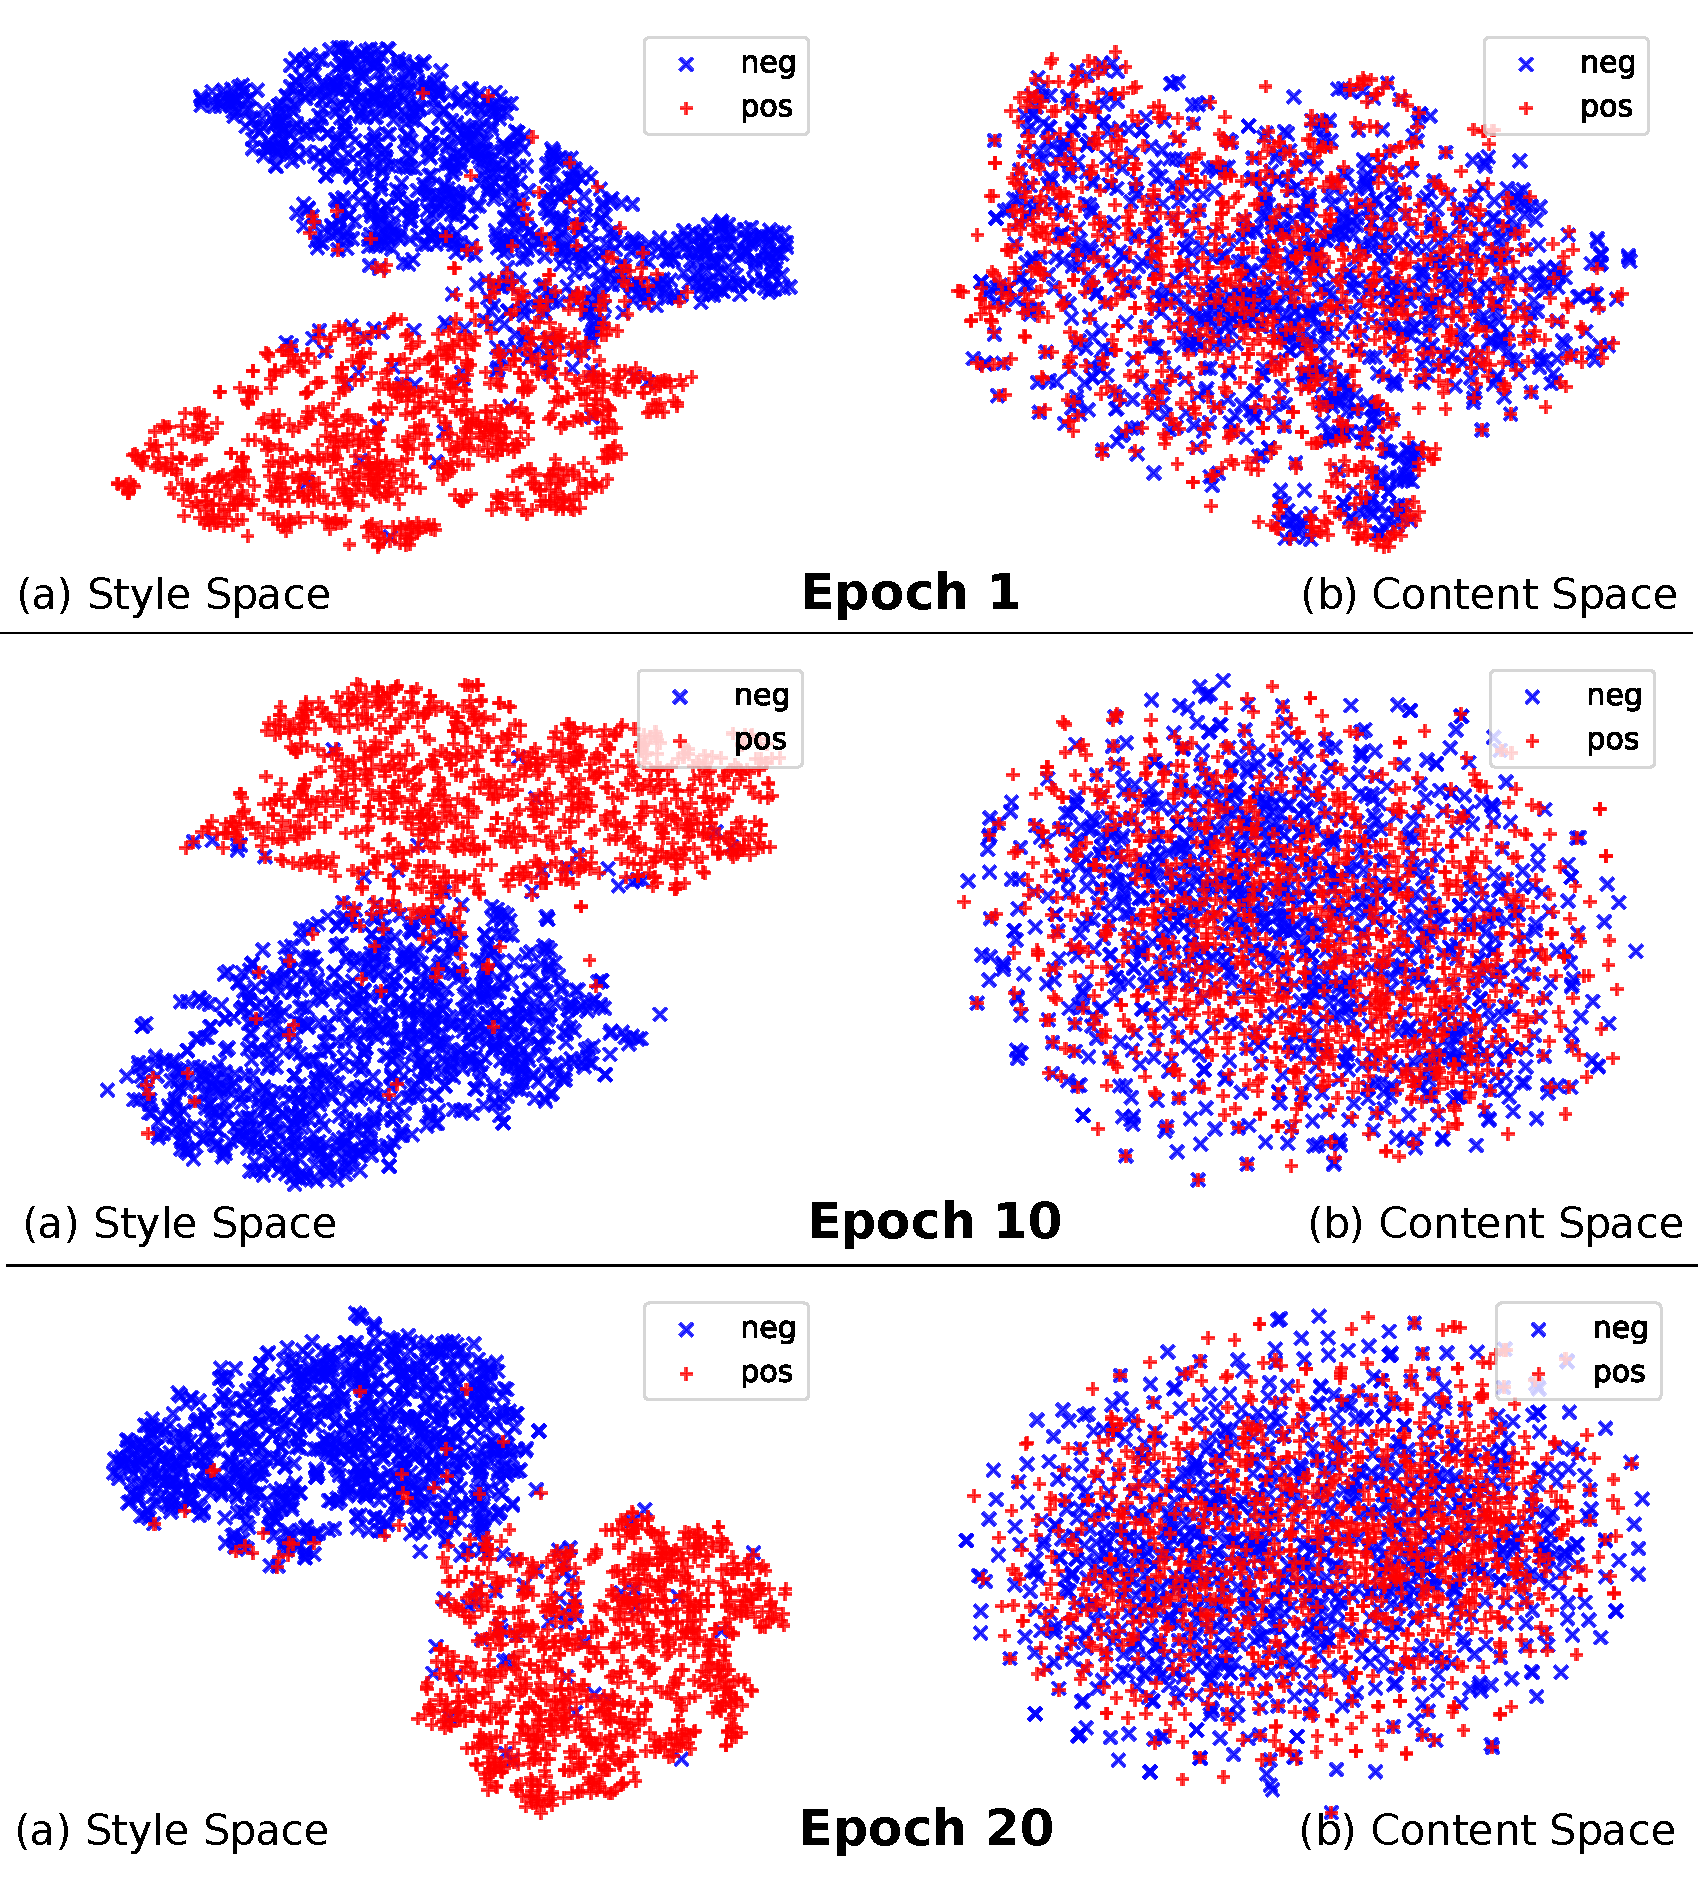
\includegraphics[width=\linewidth]{latent-spaces-vae}
	\caption{t-SNE Plots: Variational Autoencoder}
	\label{fig:vae-tsne}
\end{figure}


\subsection{Multi-Task Classification Loss} \label{ssec:multitask-classification-objective}

Our first auxiliary loss ensures the style space does contain style information. We build a classifier on the style space $\bm s$ with the objective of predicting the true style label $y'$, which is part of the training data.

This loss can be viewed as a \textit{multi-task} loss, which incentivizes the model to not only decode the sentence, but also predict its sentiment from a fixed subset of the latent variables. Similar multi-task losses are used in previous work for sequence-to-sequence learning \cite{luong2015multi}, sentence representation learning \cite{jernite2017discourse} and sentiment analysis \cite{balikas2017multitask}, among others.

In our application, we follow previous work \cite{hu2017toward,shen2017style,fu2017style} and treat the sentiment as the style of interest. We introduce a multi-label classifier
\begin{equation} \label{eqn:class-pred}
	y = \sigma(\bm w_\text{mult}^\top \bm s + b_\text{mult})
\end{equation}
where $\bm\theta_\text{mult}=[\bm w_\text{mult}; b_\text{mult}]$ are the classifier's parameters for multi-task learning, and $y$ is the predicted label distribution.

This is trained using a simple cross-entropy loss
\begin{equation} \label{eqn:multi-task-loss}
	\loss{mult}(\bm\theta_{E};\bm\theta_\text{mult}) =
	- \mathbb{E} [\log p(y' | \bm s; \bm\theta_\text{mult})]
\end{equation}
where $\bm\theta_E$ are the encoder's parameters, and $y'$ is the true label distribution.


\begin{table*}[ht]
	\centering
	\begin{tabular}{| l || c | c | c | c |}
		\hline
		\tabc{2}{Model}                      & \tabh{Transfer} & \tabh{Content}      & \tabh{Word}    & \tabh{Language} \\
		                                     & \tabh{Strength} & \tabh{Preservation} & \tabh{Overlap} & \tabh{Fluency}  \\
		\hline
		\hline
		Cross-Alignment \cite{shen2017style} & 0.809           & 0.892               & 0.209          & -23.39          \\
		\hline
		Style Embedding \cite{fu2017style}   & 0.182           & 0.959               & 0.666          & -16.17          \\
		\hline
		Ours (DAE)                           & 0.843           & 0.892               & 0.255          & -16.48          \\
		\hline
		Ours (VAE)                           & 0.890           & 0.882               & 0.211          & -14.41          \\
		\hline
	\end{tabular}
	\caption{Yelp Dataset - Comparison}
	\label{tab:yelp-comparison-previous}
\end{table*}

\begin{table*}[ht]
	\centering
	\begin{tabular}{| l || c | c | c | c |}
		\hline
		\tabc{2}{Model}                      & \tabh{Transfer} & \tabh{Content}      & \tabh{Word}    & \tabh{Language} \\
		                                     & \tabh{Strength} & \tabh{Preservation} & \tabh{Overlap} & \tabh{Fluency}  \\
		\hline
		\hline
		Cross-Alignment \cite{shen2017style} & 0.606           & 0.893               & 0.024          & -26.31          \\
		\hline
		Style Embedding \cite{fu2017style}   & 0.417           & 0.933               & 0.359          & -28.13          \\
		\hline
		Ours (DAE)                           & 0.703           & 0.918               & 0.131          & -32.42          \\
		\hline
		Ours (VAE)                           & 0.726           & 0.909               & 0.081          & -28.50          \\
		\hline
	\end{tabular}
	\caption{Amazon Dataset - Comparison}
	\label{tab:amazon-comparison-previous}
\end{table*}


\subsection{Adversarial Style Discrimination} \label{ssec:adversarial-style-objective}

The above multi-task loss only operates on the style space, but does not have an effect on the content space $\bm c$.

We therefore apply an adversarial loss to disentangle the content space from style information, inspired by adversarial generation~\cite{goodfellow2014generative}, adversarial domain adaptation~\cite{liu2017adversarial}, and adversarial style-transfer~\cite{fu2017style}.

The idea of adversarial loss is to introduce an objective that deliberately discriminates the true style label using the content vector $\bm c$. Then the autoencoder is trained to learn a content vector space that its adversary cannot predict style information from.

Concretely, the adversarial discriminator predicts style by computing a softmax distribution over the possible class labels
\begin{equation}
	y = \sigma(\bm w_\text{dis}^\top \bm c + b_\text{dis})
\end{equation}
where $\bm\theta_\text{dis}=[\bm w_\text{dis}; b_\text{dis}]$ are the parameters of the adversary, and $y$ is the predicted label distribution.

It is trained by minimizing the following objective, using a cross-entropy loss.
\begin{equation} \label{eqn:adv-disc-loss}
	\loss{dis}(\bm\theta_\text{dis}) =
	- \mathbb{E} [\log p(y' | \bm c; \bm\theta_\text{dis})]
\end{equation}
where $y'$ is the true label distribution.

The adversarial loss appears similar to the multi-task loss as in Equation \ref{eqn:multi-task-loss}. However, it should be emphasized that, for the adversary, the gradients are not propagated back to the autoencoder, i.e. the variables in $\bm c$ are treated as shallow features.

Having trained an adversary, we would like the autoencoder to be tuned in such an \textit{ad hoc} fashion, that $\bm c$ is not discriminative in style. In other words, we penalize the Shannon entropy of the adversary's prediction, given by
\begin{equation}
	\loss{adv}(\bm\theta_E)=\mathcal{H}(y|\bm c; \bm\theta_\text{dis})
\end{equation}
where $\mathcal{H}(p)=-\sum_{i\in\text{labels}}p_i\log p_i$ is the entropy and $y$ is the predicted distribution over the style labels. The adversarial objective is maximized, in this phase, with respect to the encoder. This objective helps the autoencoder maximize the uncertainty of the discriminator's predicted probability distribution.

\begin{table*}[ht]
	\centering
	\begin{tabular}{| l || c | c | c | c |}
		\hline
		\tabc{2}{Objectives}                                     & \tabh{Transfer} & \tabh{Content}      & \tabh{Word}    & \tabh{Language} \\
		                                                         & \tabh{Strength} & \tabh{Preservation} & \tabh{Overlap} & \tabh{Fluency}  \\
		\hline
		\hline
		$\loss{rec}$                                             & 0.144           & 0.915               & 0.329          & -14.28          \\
		\hline
		$\loss{rec}$, $\loss{adv}$                               & 0.727           & 0.880               & 0.204          & -14.16          \\
		\hline
		$\loss{rec}$, $\loss{mult}$                              & 0.789           & 0.898               & 0.259          & -14.56          \\
		\hline
		$\loss{rec}$, $\loss{badv}$                              & 0.168           & 0.915               & 0.328          & -14.45          \\
		\hline
		$\loss{rec}$, $\loss{adv}$, $\loss{mult}$                & 0.890           & 0.882               & 0.211          & -14.41          \\
		\hline
		$\loss{rec}$, $\loss{adv}$, $\loss{badv}$                & 0.749           & 0.883               & 0.202          & -14.36          \\
		\hline
		$\loss{rec}$, $\loss{mult}$, $\loss{badv}$               & 0.783           & 0.896               & 0.257          & -14.34          \\
		\hline
		$\loss{rec}$, $\loss{adv}$, $\loss{mult}$, $\loss{badv}$ & 0.885           & 0.878               & 0.197          & -14.05          \\
		\hline
	\end{tabular}
	\caption{Ablation Tests}
	\label{tab:ablation-results}
\end{table*}

\subsection{Adversarial Bag-of-Words Discriminator} \label{ssec:adversarial-bow-objective}

In addition to the auxiliary losses used above, we also propose a bag-of-words discriminator on the style space to make our approach complete.

The motivation is to emulate the adversarial signal provided by the style discriminator, and do the same for the content. Here, we define the content of the sentence as the words from the original sentence without any words that are discriminative of style.

The input sentences $\rmx$ are represented as vectors of the same size as the corpus vocabulary, with each index of the vector denoting the discrete probability of a word's presence in the sentence. Therefore, this bag-of-words representation is comprised of only $0$s and $1$s.

The bag-of-words discriminator uses the style vector $\bm s$ produced by the autoencoder model and tries to predict the true bag-of-words distribution using a set of parameters that are distinct from those of the autoencoder. The discriminator uses a logistic regression to predict the probability of each word's occurrence in the original sentence, between $0$ and $1$.
\begin{equation}
	b = \sigma(\bm w_\text{bow}^\top \bm s + b_\text{bow})
\end{equation}
where $\bm\theta_\text{bow}=[\bm w_\text{bow}; b_\text{bow}]$ are the classifier's parameters for bag-of-words prediction, and $b$ is the predicted word distribution.

This objective is trained in a similar method to the style adversary, using a cross-entropy loss
\begin{equation} \label{eqn:adv-bow-disc-loss}
	\loss{bow}(\bm\theta_\text{bow}) =
	- \mathbb{E} [\log p(b' | \bm s; \bm\theta_\text{bow})]
\end{equation}
where $b'$ is the true word distribution.

We also refrain from propagating the effects of this discriminator loss $\loss{bow}$ to the encoder parameters, ensuring that the parameters that each adversary and the autoencoder can update are mutually exclusive.

Similar to the style adversary, the empirical Shannon entropy of the predicted distribution is provided as a training signal for the autoencoder model to maximize.
\begin{equation}
	\loss{badv}(\bm\theta_E) = \mathcal{H}(b | \bm s; \bm\theta_\text{bow})
\end{equation}
where $b$ is the predicted word distribution.

The motivation for this adversarial loss is similar to the one used in the context of the style discriminator. We want to encourage the encoder to learn a representation of style $\bm s$ that the bag-of-words discriminator cannot predict most of the original words from.

\subsection{Training Process}

The overall loss $\loss{ovr}$, used for the autoencoder, is thus comprised of four distinct objectives: the reconstruction objective, the multi-task objective, and the adversarial objectives for style and content.
\begin{align*}
	\loss{ovr} =
	 & \loss{rec}(\bm\theta_E, \bm\theta_D) - \lambda_\text{adv} \loss{adv}(\theta_E) +                                \\
	 & \lambda_\text{mult} \loss{mult} (\bm\theta_E,\bm\theta_\text{mult}) - \lambda_\text{badv} \loss{badv}(\theta_E)
\end{align*}
where $\lambda_\text{mult}$, $\lambda_\text{adv}$ and $\lambda_\text{badv}$ balance the model's auxiliary losses.

To put it all together, the model training consists of a loop involving the processes as shown in Algorithm \ref{alg:training-process}.
\begin{algorithm}[ht]
	\While{epochs remaining}{
		minimize $\loss{dis}(\bm\theta_\text{dis})$ w.r.t. $\bm\theta_\text{dis}$\;
		minimize $\loss{bow}(\bm\theta_\text{bow})$ w.r.t. $\bm\theta_\text{bow}$\;
		minimize $\loss{ovr}$ w.r.t. $\bm\theta_E, \bm\theta_D, \bm\theta_\text{mult}$\;
	}
	\caption{Training Process}
	\label{alg:training-process}
\end{algorithm}

We use the Adam optimizer \cite{kingma2014adam} for the autoencoder and the RMSProp optimizer \cite{tieleman2012lecture} for the discriminators, each with an initial learning rate of $10^{-3}$, and train the model for 20 epochs. Both the autoencoder and the discriminators are trained once per epoch with $\lambda_\text{mult} = 1$, $\lambda_\text{adv} = 0.3$ and $\lambda_\text{badv} = 0.001$. The recurrent unit size is $256$, the style vector size is $8$, and the content vector size is $128$. We append the latent vector $\bm h$ to the hidden state at every time step of the decoder \cite{bahuleyan2017variational}. For the VAE model, we set $\lambda_{\text{skl}} = 0.03$ and $\lambda_{\text{ckl}} = 0.03$ and use the $\operatorname{sigmoid}$ KL-weight annealing schedule proposed by \citeay{bahuleyan2018probabilistic}.


\subsection{Generating Style-Transferred Sentences} \label{ssec:sentence-generation}

A direct application of our disentangled latent space is style-transfer for natural language generation. For example, we can generate a sentence with generally the same meaning (content) but a different style (e.g. sentiment).

Let $\rmx^*$ be an input sentence with $\bm s^*$ and $\bm c^*$ being the encoded, disentangled style and content vectors, respectively. If we would like to transfer its content to a different style, we compute an empirical estimate of the target style's vector $\hat{\bm s}$ by
\begin{equation*}
	\hat{\bm s}=\frac{\sum_{i\in\text{target style}}\bm s_i}{\text{\# target style samples}}
\end{equation*}
The inferred target style $\hat{\bm s}$ is concatenated with the encoded content $\bm c^*$ for decoding style-transferred sentences (Figure~\ref{fig:model-inference-overview}).

\begin{table*}[ht]
	\centering
	\begin{tabular}{| p{0.3\linewidth} || p{0.3\linewidth} | p{0.3\linewidth} |}
		\hline
		\tabc{2}{Original (Positive)}                                   & \tabh{DAE Transferred}                                                  & \tabh{VAE Transferred}                                               \\
		                                                                & \tabh{(Negative)}                                                       & \tabh{(Negative)}                                                    \\
		\hline
		\hline
		\textit{i would recommend a visit here}                         & \textit{i would not recommend this place again}                         & \textit{i would not recommend this place for my experience}          \\
		\hline
		\textit{the restaurant itself is romantic and quiet}            & \textit{the restaurant itself is soooo quiet}                           & \textit{the restaurant itself was dirty}                             \\
		\hline
		\textit{my experience was brief but very good}                  & \textit{my experience was very loud and very expensive}                 & \textit{my experience was ok but not very much}                      \\
		\hline
		\textit{the food is excellent and the service is exceptional}   & \textit{the food is by the worst part is the horrible costumer service} & \textit{the food was bland and i am not thrilled with this}          \\
		\hline
		\textit{the food is very very amazing like beef and fish}       & \textit{the food is very horrible i have ever had mostly fish}          & \textit{the food is very bland and just not fresh}                   \\
		\hline
		\textit{we will definitely come back here}                      & \textit{we will not come back here again}                               & \textit{we will never come back here}                                \\
		\hline
		\textit{both were very good}                                    & \textit{everything was very bland}                                      & \textit{both were very bad}                                          \\
		\hline
		\hline
		\hline
		\tabc{2}{Original (Negative)}                                   & \tabh{DAE Transferred}                                                  & \tabh{VAE Transferred}                                               \\
		                                                                & \tabh{(Positive)}                                                       & \tabh{(Positive)}                                                    \\
		\hline
		\hline
		\textit{so nasty}                                               & \textit{so helpful}                                                     & \textit{so fabulous}                                                 \\
		\hline
		\textit{consistently slow}                                      & \textit{consistently awesome}                                           & \textit{fast service}                                                \\
		\hline
		\textit{crap fries hard hamburger buns burger tasted like crap} & \textit{cheap and yummy sandwiches really something different}          & \textit{yummy hamburgers and blue cheese bagels are classic italian} \\
		\hline
		\textit{oh and terrible tea}                                    & \textit{oh and awesome tea}                                             & \textit{oh and great tea}                                            \\
		\hline
		\textit{the interior is old and generally falling apart}        & \textit{the interior is clean and orderly as entertaining}              & \textit{the interior is old and noble}                               \\
		\hline
		\textit{front office customer service does not exist here}      & \textit{front office is very professional does you}                     & \textit{kudos to customer service is very professional}              \\
		\hline
		\textit{the crust was kinda gooey like}                         & \textit{the crust is kinda traditional}                                 & \textit{the crust is soooooo worth it}                               \\
		\hline
	\end{tabular}
	\caption{Examples of Style-Transfer Generation}
	\label{tab:transfer-samples}
\end{table*}

\section{Experiments}

\subsection{Datasets}

We conduct experiments on two datasets, the details for which are given below. Both of these datasets are comprised of sentences accompanied by binary sentiment labels (positive, negative) and are, therefore, used to evaluate the task of sentiment transfer.

\subsubsection{Yelp Service Reviews}

We use a Yelp review dataset \cite{challenge2013yelp}, which has been sourced from the code repository accompanying the implementation of the paper by \citeay{shen2017style}~\footnote{\url{https://github.com/shentianxiao/language-style-transfer}}. It contains 444101, 63483 and 126670 sentences for train, validation, and test, respectively. The maximum sentence length is 15, and the vocabulary size is about 9200.

\subsubsection{Amazon Product Reviews}

We also use an Amazon product reviews dataset~\footnote{\url{http://jmcauley.ucsd.edu/data/amazon/}}, following \citeay{fu2017style}. The reviews were sourced from the code repository accompanying the paper~\footnote{\url{https://github.com/fuzhenxin/text_style_transfer}}. It contains 559142, 2000 and 2000 sentences for train, validation, and test, respectively. The maximum sentence length is 20, and the vocabulary size is about 58000.

\subsection{Evaluation Metrics}

We evaluate our method using four metrics: style-transfer strength, content preservation, word overlap, and language fluency.

\subsubsection{Style-Transfer Strength}
We train a convolutional neural network (CNN) style classifier \cite{kim2014convolutional} and predict the style of the generated sentences. While the style classifier itself may not be perfect, it provides a quantitative way of evaluating the strength of style-transfer \cite{hu2017toward,shen2017style,fu2017style}. The validation accuracies of the sentiment classifier trained on the Yelp and Amazon datasets are $\approx 0.97$ and $\approx 0.82$, respectively. The classifier accuracy on the style-transferred sentences, considering the target style to be the true label, is reported as the style-transfer strength.

\subsubsection{Content Preservation}
We compute a sentence embedding by min, max, and average pooling its constituent word embeddings. Then, the cosine similarity between the source and generated sentence embedding is computed to evaluate how close they are in meaning. Here, sentiment words from a stop list \cite{hu2004mining} are removed \cite{fu2017style}. The cosine similarity is reported as the content preservation score.

\subsubsection{Word Overlap}
We also utilize a simpler unigram overlap metric to evaluate the similarity between the source and generated sentences. Given a source sentence $x$ and an attribute style-transferred sentence $y$, let $w_x$ and $w_y$ be the set of unique words present in $x$ and $y$ respectively, while excluding sentiment words \cite{hu2004mining} and stopwords \cite{bird2004nltk}. Then, the word overlap score can be calculated using $$\operatorname{word-overlap} = \frac{count(w_x \cap w_y)}{count(w_x \cup w_y)}$$ which is simply a normalized measure of overlapping unigrams in the source and target sentences.

\subsubsection{Language Fluency}
We use a trigram Kneser-Ney smoothed language model \cite{kneser1995improved} as a quantifiable and automated scoring metric by which to assess the quality of generated sentences. It calculates the probability distribution of trigrams in a corpus, based on their occurrence statistics, to build a language model. We train this language model on the complete corpus that we evaluate our style-transfer models with. The log-likelihood score for a generated sentence, as predicted by the Kneser-Ney language model, is reported as the indicator of language fluency.

\subsubsection{Manual Evaluation of Language Quality}
We perform manual evaluations by randomly sampling sentences generated from each model trained on the Yelp dataset, and requesting 5 human annotators to rate them on a 1-5 Likert scale \footnote{5=Flawless, 4=Good, 3=Adequate, 2=Poor, 1=Incomprehensible} \cite{stent2005evaluating} based on their syntax, grammar and fluency. The aggregate score of all the evaluators is reported as a measure of language quality.


\section{Discussion}

\subsection{Disentangling Latent Space}

We first analyze how the style (sentiment) and content of the latent space are disentangled. We train classifiers on the different latent spaces, and report their inference-time classification accuracies in Table~\ref{tab:classification}. These are results from the experiments on the Yelp dataset.

\begin{table}[ht]
	\centering
	\begin{tabular}{| l || r | r |}
		\hline
		\textit{Random/Majority guess}   & \multicolumn{2}{c|}{0.602}              \\ \hline \hline
		\hline
		\tabc{1}{Latent Space}           & \tabh{DAE}                 & \tabh{VAE} \\
		\hline \hline
		Content space  ($\bm c$)         & 0.614                      & 0.657      \\ \hline
		Style space ($\bm s$)            & 0.793                      & 0.791      \\ \hline
		Complete space ($[\bm s;\bm c]$) & 0.792                      & 0.792      \\
		\hline
	\end{tabular}
	\caption{Style Classification Accuracy}
	\label{tab:classification}
\end{table}

We see that the 128-dimensional content vector $\bm c$ is not particularly discriminative for style. It achieves accuracies that are only slightly better than random/majority guess. However, the 8-dimensional style vector $\bm s$, despite its low dimensionality, achieves significantly higher style classification accuracy. When combining content and style vectors, we achieve no further improvement. These results verify the effectiveness of our disentangling approach, because the style space does contain style information, whereas the content space does not.

We show t-SNE plots of both the deterministic autoencoder (DAE) and the variational autoencoder (VAE) models in Figure \ref{fig:dae-tsne} and Figure \ref{fig:vae-tsne}, respectively. As can be seen from the t-SNE plots, sentences with different styles are noticeably separated in a cleaner manner in the style space (LHS), but are indistinguishable in the content space (RHS). It is also evident that the latent space learned by the variational autoencoder is considerably smoother and continuous compared to the one learned by the deterministic autoencoder.


\subsection{Style-Transfer Sentence Generation}

We apply the disentangled latent space to a style-transfer sentence generation task, where the goal is to generate a sentence with different sentiment. We compare our approach with previous state-of-the-art work in Table~\ref{tab:yelp-comparison-previous} and Table~\ref{tab:amazon-comparison-previous}. We replicated the experiments with their publicly available code and data.

We observe that the style embedding model \cite{fu2017style} performs poorly on the style-transfer objective, resulting in inflated content preservation and word overlap scores. A qualitative analysis indicates that this model resorts to simply reconstructing most of the source sentences, and is not very effective at transferring style.

Results show that, our approach achieves comparable content preservation and word overlap scores to previous work \cite{shen2017style}, and significantly better style-transfer strength scores than either of the models compared to, showing that our disentangled latent space can be used for better style-transfer sentence generation. Our VAE model also produces the most fluent sentences for the Yelp dataset task, which is corroborated by the manual evaluation results.

Table~\ref{tab:ablation-results} presents the results of an ablation test. We see that both the style adversarial loss and multi-task classification loss play a role in the strength of style-transfer, and that they can be combined to further improve performance. Also, the combination of all the losses described yields the best language fluency score. We observe that the bag-of-words adversary described in Section \ref{ssec:adversarial-bow-objective} does not provide much of an improvement in terms of our evaluation metrics. However, this idea can be improved upon in future work.

\begin{table}[ht]
	\centering
	\begin{tabular}{| l || c |}
		\hline
		\tabc{2}{Model}                      & \tabh{Language} \\
		                                     & \tabh{Quality}  \\
		\hline
		\hline
		Cross-Alignment \cite{shen2017style} & 3.188           \\
		\hline
		Style Embedding \cite{fu2017style}   & 3.784           \\
		\hline
		Ours (DAE)                           & 3.460           \\
		\hline
		Ours (VAE)                           & 3.824           \\
		\hline
	\end{tabular}
	\caption{Results - Manual Evaluation}
	\label{tab:manual-evaluation}
\end{table}

The manual evaluation results are presented in Table \ref{tab:manual-evaluation}. Our VAE model attains the best score for generated sentence quality amongst all the evaluated models. We also observe that the ranking of these models is positively correlated with the automated `Language Fluency' metric presented in Table \ref{tab:yelp-comparison-previous}.

Some examples of style-transfer sentence generation are presented in Table~\ref{tab:transfer-samples}. We see that, with the empirically estimated style vector, we can reliably control the sentiment of generated sentences.


\section{Conclusion and Future Work}
In this paper, we propose a simple yet effective approach for disentangling the latent space of neural networks using multi-task and adversarial objectives. Our learned disentanglement approach can be applied to text style-transfer tasks. It achieves similar content preservation scores, and significantly better style-transfer strength scores compared to previous state-of-the-art work.

For future work, we intend to evaluate the effects of disentangling the style space for datasets with greater than two distinct styles. We would also like to explore the possibility of aligning each encoded style distribution to a unique prior, which could be sampled from at inference time for style-transfer, as opposed to using the empirical mean of training-time style embeddings.

\section{Acknowledgements}
We acknowledge the support of the Natural Sciences and Engineering Research Council of Canada (NSERC) [261439-2013-RGPIN], and Amazon Research Award. The Titan Xp GPU used for this research was donated by the NVIDIA Corporation.


\bibliography{main}
\bibliographystyle{aaai}

\end{document}
